\documentclass[xetex,mathserif,serif]{beamer}
\usepackage{polyglossia}
\setdefaultlanguage[babelshorthands=true]{russian}
\usepackage{minted}
\usepackage{tabu}

\useoutertheme{infolines}

\usepackage{fontspec}
\setmainfont{FreeSans}
\newfontfamily{\russianfonttt}{FreeSans}

\definecolor{links}{HTML}{2A1B81}
\hypersetup{colorlinks,linkcolor=,urlcolor=links}

\tabulinesep=0.7mm

\newcommand{\attribution}[1] {
    \vspace{-5mm}\begin{flushright}\begin{scriptsize}\textcolor{gray}{\textcopyright\, #1}\end{scriptsize}\end{flushright}
}

\title{Практика 8: Развёртывание, Docker}
\author[Юрий Литвинов]{Юрий Литвинов \newline \textcolor{gray}{\small\texttt{yurii.litvinov@gmail.com}}}

\date{26.05.2020г}

\begin{document}
    
    \frame{\titlepage}

    \section{Docker}

    \begin{frame}
        \frametitle{Docker}
        \begin{itemize}
            \item Средство для ``упаковки'' приложений в изолированные контейнеры
            \item Что-то вроде легковесной виртуальной машины
        \end{itemize}
        \begin{center}
            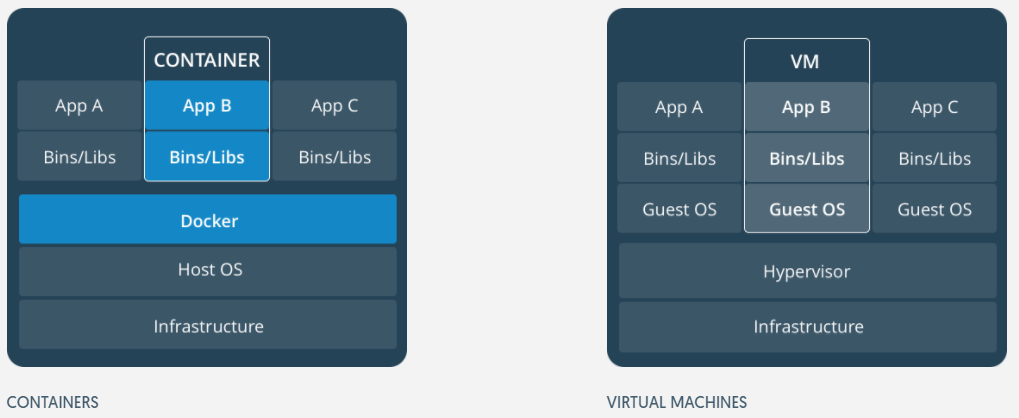
\includegraphics[width=0.7\textwidth]{docker.png}
            \attribution{\url{https://www.docker.com}}
        \end{center}
    \end{frame}
    
    \begin{frame}[fragile]
        \frametitle{Dockerfile}
        \begin{scriptsize}
            \begin{minted}{sh}
# Use an official Python runtime as a parent image
FROM python:2.7-slim

# Set the working directory to /app
WORKDIR /app

# Copy the current directory contents into the container at /app
ADD . /app

# Install any needed packages specified in requirements.txt
RUN pip install --trusted-host pypi.python.org -r requirements.txt

# Make port 80 available to the world outside this container
EXPOSE 80

# Define environment variable
ENV NAME World

# Run app.py when the container launches
CMD ["python", "app.py"]
            \end{minted}
        \end{scriptsize}
    \end{frame}

    \begin{frame}[fragile]
        \frametitle{Балансировка нагрузки}
        \framesubtitle{docker-compose.yml}
        \begin{scriptsize}
            \begin{minted}{yaml}
version: "3"
services:
    web:
        # replace username/repo:tag with your name and image details
        image: username/repo:tag
        deploy:
            replicas: 5
            resources:
                limits:
                    cpus: "0.1"
                    memory: 50M
            restart_policy:
                condition: on-failure
        ports:
            - "80:80"
        networks:
            - webnet
networks:
    webnet:
            \end{minted}
        \end{scriptsize}
    \end{frame}

    \begin{frame}
        \frametitle{Swarm-ы}
        \begin{itemize}
            \item Машина, на которой запускается контейнер, становится главной
            \item Другие машины могут присоединяться к swarm-у и получать копию контейнера
            \item Docker балансирует нагрузку по машинам
        \end{itemize}
        \begin{center}
            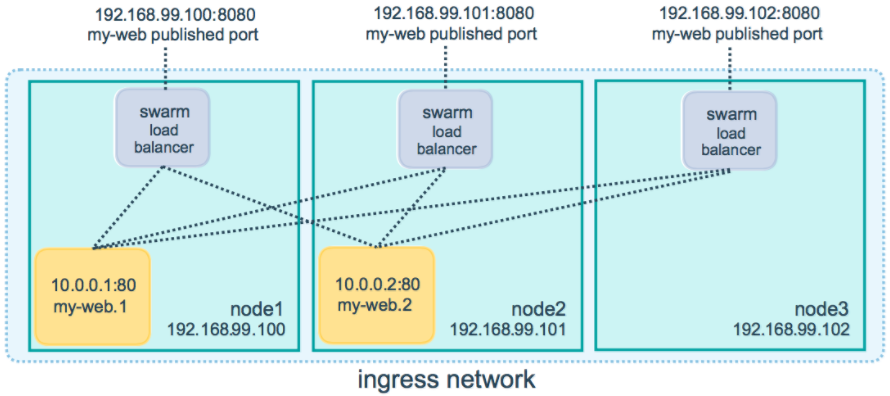
\includegraphics[width=0.7\textwidth]{swarmLoadBalancing.png}
            \attribution{\url{https://www.docker.com}}
        \end{center}
    \end{frame}

    \section{Задача}

    \begin{frame}
        \frametitle{Задание на пару}
        В командах по два человека оформить сетевой чат, разработанный на предыдущем занятии, в виде Docker-контейнера
        \begin{itemize}
            \item Убедиться, что при запуске клиента и сервера через Docker они могут установить соединение
            \item Выложить в свой репозиторий Docker-файл
        \end{itemize}
    \end{frame}

    \begin{frame}
        \frametitle{Что делать}
        \begin{itemize}
            \item Заполнить форму \url{https://forms.gle/fTaEJ2YQaBHUNmnZ6} ссылками на репозиторий и командный чат
            \begin{itemize}
                \item Сделать это в самом начале работы
            \end{itemize}
            \item Выложить на HwProj результаты к концу пары
            \item Доделать ``дома'', если не успели
        \end{itemize}
    \end{frame}

\end{document}